\subsection{Subsystem 3: Text Display \& Chassis}

% Subsystem Diagram
\subsubsection{Subsystem Diagrams}
\begin{figure}[h]
    \centering
    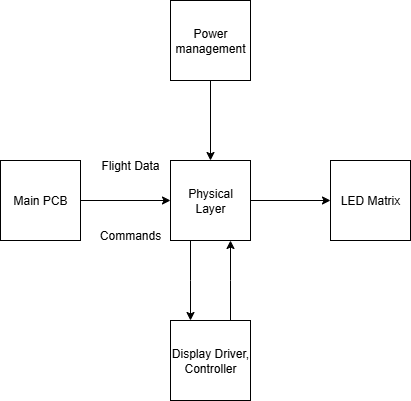
\includegraphics[width=12cm]{images/blockDiagram-display.png} % Change the picture
    \caption{Subsystem Block Diagram}
\end{figure} % If your subsystem is more coding, change it to activity diagram

% Specifications
\subsubsection{Specifications}
\begin{enumerate}
    \item Feature a 2056-pixel Dot Display (128 x 256px)
    \item Physical dimensions of housing within 5\% of 64 x 128 x 256 mm.
\end{enumerate}

% Subsystem Interactions
\subsubsection{Subsystem Interactions}
The display subsystem links the main PCB and the LED Matrix. This subsystem will interface with the power management system and the main PCB. It will recieve data and commands from the main PCB, interpret the commands, and display the data.

% Core ECE
\subsubsection{Core ECE Design Tasks}
\begin{itemize}
    \item \textbf{ECE 27000}: Provides a solid foundation in logic circuits. Helps for designing registers, data paths, logic that drives the LED panel.
    \item \textbf{ECE 25500}: Provides a base understanding of transisters, amplifiers, and fundamentals into I-V behavior.
    \item \textbf{ECE 40862}: Teaches valuable STM concepts such as programming, interrupts, and DMA which are needed to drive the display controller efficiently.
\end{itemize}

% Schematics
\subsubsection{Schematics}
[Type here \textbf{DD2+}]
\begin{figure}[h]
    \centering
    
\includegraphics[width=16cm]{images/white.png} % Change the picture
    \caption{[Schematic Name]}
\end{figure} % If your subsystem is more coding, change it to psudo code

% Parts List
\subsubsection{Parts}
\begin{itemize}
    \item {[Type here \textbf{DD1+}]}
    \item 32 x 64 px LED Matrix (ADAFruit from DigiKey)
    \item 
\end{itemize}

% Algorithm
\subsubsection{Algorithm}

\begin{lstlisting}
    Initialize:
    Configure GPIOs for DATA, CLK, LAT, OE, row select lines (A,B,C,D)
    Initialize interface for incoming data
    Initialize timer for refresh interrupts
    Set PWM resolution (e.g., 8-bit)

    Main Loop:
    while (true):
        if new frame data available from main PCB:
            copy frame buffer into local memory (double buffer optional)
        
        for each row_index in 0 .. NUM_ROWS-1:
            select_row(row_index)        
            OE = HIGH                   
            
            for pwm_bit = 7 downto 0:    // for 8-bit PWM
                for col_index = 0 .. NUM_COLS-1:
                    pixel = frame_buffer[row_index][col_index]
                    if pixel.red  & (1 << pwm_bit) != 0:
                        DATA_R = HIGH
                    else:
                        DATA_R = LOW
                    if pixel.green & (1 << pwm_bit) != 0:
                        DATA_G = HIGH
                    else:
                        DATA_G = LOW
                    if pixel.blue & (1 << pwm_bit) != 0:
                        DATA_B = HIGH
                    else:
                        DATA_B = LOW
                    
                    pulse(CLK)           
                    
                pulse(LAT)                
                OE = LOW                   
                delay(PWM_DELAY[pwm_bit])  
                
        repeat indefinitely
\end{lstlisting}

% Theory of Operation
\subsubsection{Theory of Operation}
[Type here \textbf{DD2+}]

% Specification Measurement
\subsubsection{Specifications Measurement}
[\textbf{DD3+} Every specification here should match the specification above. ]
\begin{enumerate}
    \item {[Copy specification here. ]} \\
          {[Explain the specification here. Add photoes if necessary. ]}
\end{enumerate}

% Standards
\subsubsection{Standards}
[\textbf{DD1+}]
\begin{itemize}
    \item \textbf{[Standard Name]}: [Describe the standards and explain the connection]
\end{itemize}